\onecolumn
\thispagestyle{empty}
\newgeometry{top=2.5cm, left=2.5cm, right=3.9cm, bottom=1cm}
 
\begin{wrapfigure}{l}{0.4\columnwidth}
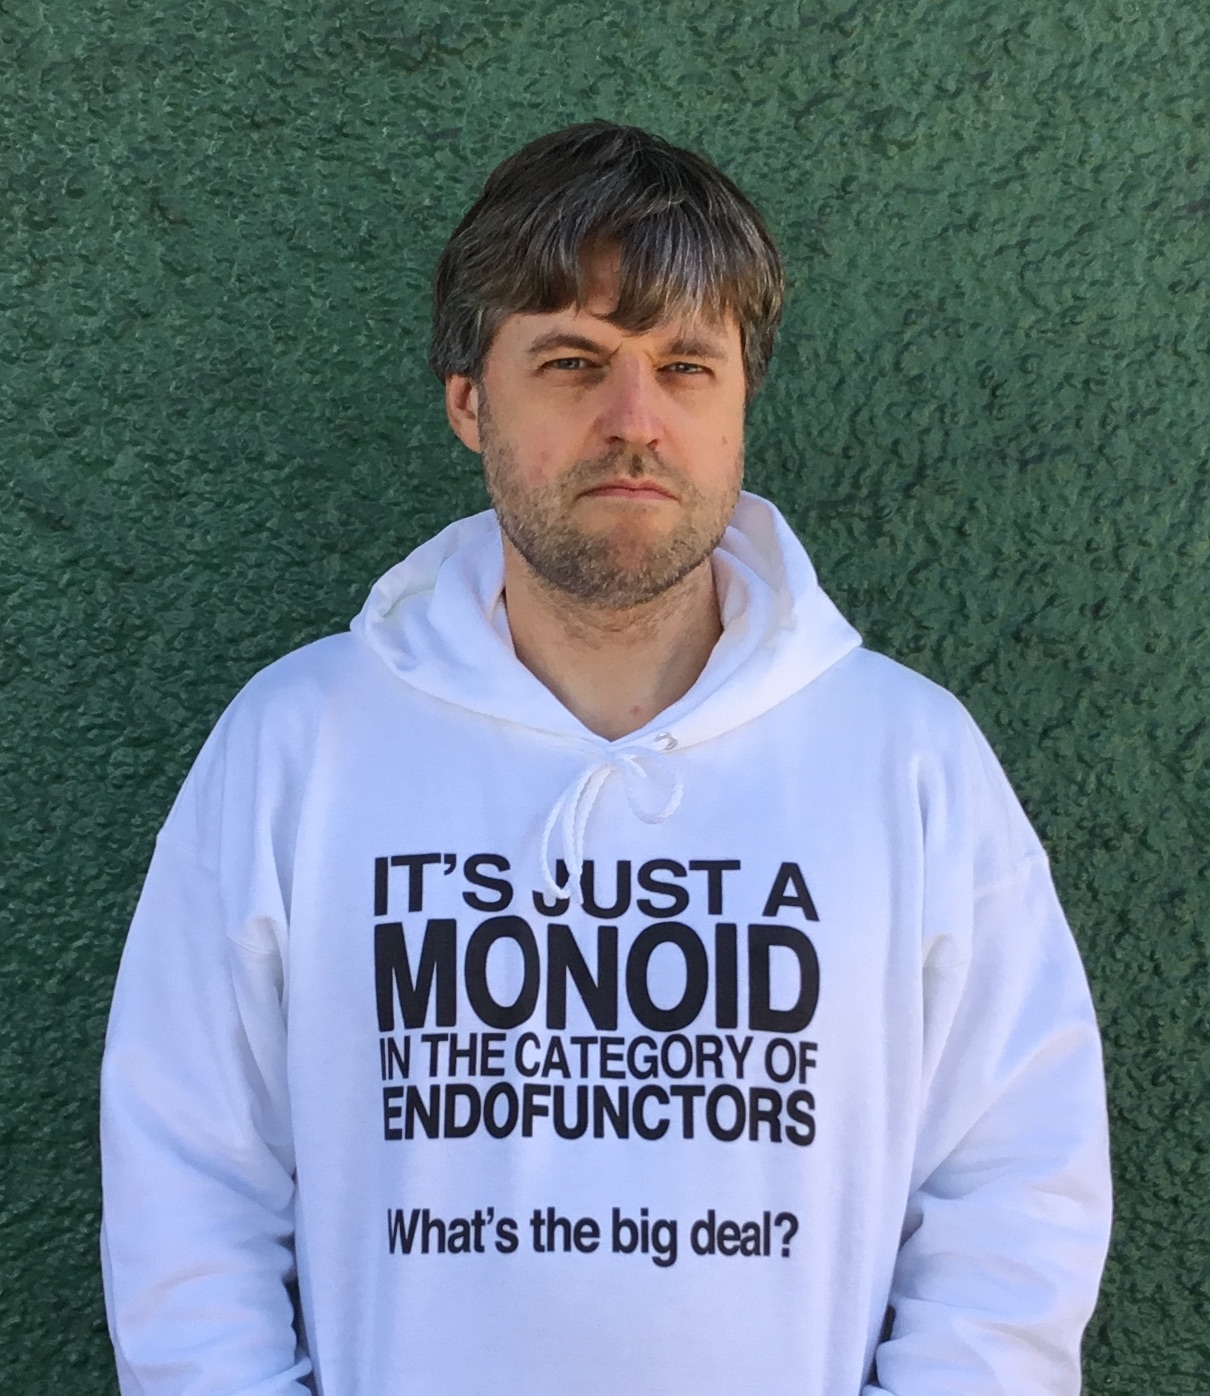
\includegraphics[width=0.4\columnwidth]{monads_evil_face}
\vspace{-2.0\baselineskip}
\end{wrapfigure}

%\noindent
\smaller
This book is a pedagogical in-depth tutorial and reference
on the theory of functional programming (FP) as practiced in the early
21$^{\text{st}}$ century. Starting from issues found in practical
coding, the book builds up the theoretical intuition, knowledge, and
techniques that programmers need for rigorous reasoning about types
and code. Examples are given in Scala, but most of the material applies equally
to other FP languages.

The book\textsf{'}s topics include working with FP-style collections; reasoning about recursive
functions and types; the Curry-Howard correspondence; laws, structural
analysis, and code for functors, monads, and other typeclasses based on exponential-polynomial data types; 
techniques of symbolic derivation and proof;
free typeclass constructions; and
practical applications of parametricity.

Long and difficult, yet boring explanations are logically
developed in excruciating detail through 1982
Scala code snippets, 233 statements with step-by-step
derivations, 105 diagrams, 237 examples
with tested Scala code, and 315 exercises. Discussions
build upon each chapter\textsf{'}s material further.

Beginners in FP will find tutorials about the \texttt{map}/\texttt{reduce}
programming style, type parameters, disjunctive types, and higher-order
functions. For more advanced readers, the book shows  the practical
uses of the Curry-Howard correspondence and the parametricity theorems
without unnecessary jargon; proves that all the standard monads (e.g.,
\texttt{List} or \texttt{State})
satisfy the monad laws; derives lawful instances of \texttt{Functor}
and other typeclasses from types; shows that monad transformers need
18 laws;
and explains the use of parametricity for reasoning about the Church encoding and the free typeclasses.

Readers should have a working knowledge of programming; e.g.,
be able to write code that prints the number of distinct words in
a sentence. The difficulty of this book\textsf{'}s mathematical derivations
is at the level of undergraduate multivariate calculus, similar to that of multiplying
matrices or simplifying the expressions:
\[
\frac{1}{x-2}-\frac{1}{x+2}\quad\text{ and }\quad\frac{d}{dx}\left((x+1)f(x)e^{-x}\right)\quad.
\]

The author received a Ph.D. in theoretical physics. After a career in academic research, he works as a software engineer.


%\vspace{3.0cm}\hspace*{\fill}\colorbox{white}{\includegraphics[scale=1.0,width=50.8mm,height=30.5mm]{barcode}}
